\begin{flushleft}
    \textit{Technologischer Standpunkt Software:}\\
    (TODO React???)
    ROS bietet bereits ein starkes und recht einfach nutzbares Framework, allerdings vermisst man eine 
    schöne und einfach bedienbare graphische Oberfläche.
    Es existieren kleinere Projekte welche sich dieser Frontend entwicklung annehmen. 
    Allerdings hat uns keines dieser Projekte zufrieden gestellt. 
    Vor allem was die Orchestrierungsmöglichkeit mehrerer Roboter angeht.

    \begin{description}
        \item[Robotik:]\hfill\\
        \begin{flushleft}
    Ganz klar werden hier die Begriffe \textit{Roboter} und \textit{Robotik} voneinander getrennt.
    Wo der Begriff \textit{Roboter} klar definiert ist und unter strengen Richtlinien und Normen steht, die beschreiben, was ein Roboter ist, da ist der Begriff der \textit{Robotik} nicht genau definiert.
    
    Jedoch versteht man in der Robotik die Steuerung und Anwendung von Robotersystemen.
    Ganz gleich können hier Industrie- und Serviceroboter mit in Verbindung gebracht werden.
    Ein wichtiges Merkmal hierfür ist die Interaktion mit der physischen Welt, wofür ein Roboter Aktoren und Sensoren benutzt.
    Die Robotik ist eine interdisziplinäre Wissenschaft, da sie Gebiete der Informatik, Maschinenbau, Elektronik und der Mathematik vereint. 
    \cite{robotik_konradin}

    Als eines des bekanntesten und meist verbreitetsten Frameworks zur Steuerung von Robotern ist ROS (Robot Operating System), auf das im Folgenden Kapitel der Grundbegriffe genauer eingegangen wird.

\end{flushleft}

        \item[ROS:]\hfill\\
        ROS steht für Robot Operating System. Das "Operating System" ist kein richtiges Betriebssystem sondern eine Sammlung von Softwarebibliotheken, die es einem vereinfachen Robotiksysteme zu bauen.
        Der Kern von ROS besteht aus Interfaces, genannt ROS-Graph, die eine anonymisierte und standardisierte Interprozesskommunikation ermöglichen.
        Dieser Graph ist ein Netzwerk aus 'nodes', welche über 'topics' miteinander kommunizieren. 'Nodes' werden als Prozesse auf einem oder verschiedenen Computern ausgeführt.
        Auf einem 'topic' wird immer dieselbe 'message' mit einem definierten Datentyp von 'nodes' verbreitet. 
        Für das Verbreiten und Empfangen von Messages müssen die Nodes 'publisher' und 'subscriber'-Interfaces implementieren.
        In Abbildung \ref{fig:ros_graph} kann man einen ROS-Graph sehen, der aus zwei Nodes besteht, die über ein Topic miteinander kommunizieren.
        In diesem Fall gibt es einen publisher der Nachrichten sendet und einen subscriber der Nachrichten empfangen kann.

        \begin{figure}[h!]
            \centering
            
\includegraphics[width=0.8\textwidth]{imgs/Grundbegriffe/graph_2_nodes_with_topic.png}
            \caption{Beispiel ROS Graph}
            \label{fig:ros_graph}%
        \end{figure}

        Des weiteren gibt es noch viele Tools, die wie zum Beispiel in Abbildung \ref{fig:ros_graph} den ROS-Graph visualisieren können, und eine große Menge an Bibliotheken, welche Standard-Algorithmen der Robotik implementieren.
        Diese Tools und Bibliotheken werden ebenfalls zu ROS gezählt weshalb ROS als mehr als ein Framework angesehen wird.

        Es gibt eine ältere Version von ROS die einfach nur ROS genannt wird und eine neuere Version namens ROS2.
        Der Hauptunterschied zwischen ROS und ROS2 ist, dass ROS einen zentralen Server, genannt 'ROS-Master' verwendet und ROS2 einen dezentralen Ansatz verfolgt.
        Der 'ROS-Master' besteht im Kern aus einer Datenbank in der die Teilnehmer der verschiedenen Topics aufgelistet werden und in der die Teilnehmer des Netzwerks ihre entsprechenden Partner finden können, mit denen sie eine TCP-Verbindung aufbauen.
        
        ROS2 baut auf dem Data-Distribution Service Standard von OMG auf. 
        Das ist eine Spezifikation für eine Middleware, welche ein 'Data-Centric Subscriber-Publisher (DCPS)'-Modell beschreibt und somit sehr ähnlich zu dem ROS-Graphen ist. 
        Die Middleware stellt die Peer-to-Peer Funktionalität auf Basis von UDP zur Verfügung.

        \item[Micro-ROS]\hfill\\
        Micro-ROS ist eine Kombination von einem RTOS, einer Client-Bibliothek, einer Middleware und einem sogenannten ROS2 Agent, 
        die Mikrocontroller möglichst effizient in das ROS-Oekosystem einbinden soll.
        
        Mit Micro-ROS ist es nicht möglich ROS-messages direkt im Netzwerk zu versenden und mit anderen Teilnehmern direkt in Verbindung zu stehen.
        Die dafür benötigte Middleware würde zu viele Ressourcen auf einem Mikrocontroller verbrauchen. 
        Stattdessen gibt es einen sogenannten ROS-Agent, mit dem sich der Mikrocontroller mit Hilfe einer für Mikrocontroller optimierten Middleware verbindet.
        Der ROS-Agent ist dann im Prinzip eine Brücke zwischen den verschiedenen Middlewares, wie man in Abbildung \ref{fig:micro-ros-architecture} sehen kann. Entsprechend muss der Agent auch auf leistungsfähigerer Hardware ausgeführt werden.    
        \cite{micro_ros_concepts}
        \begin{figure}[h!]
            \centering
            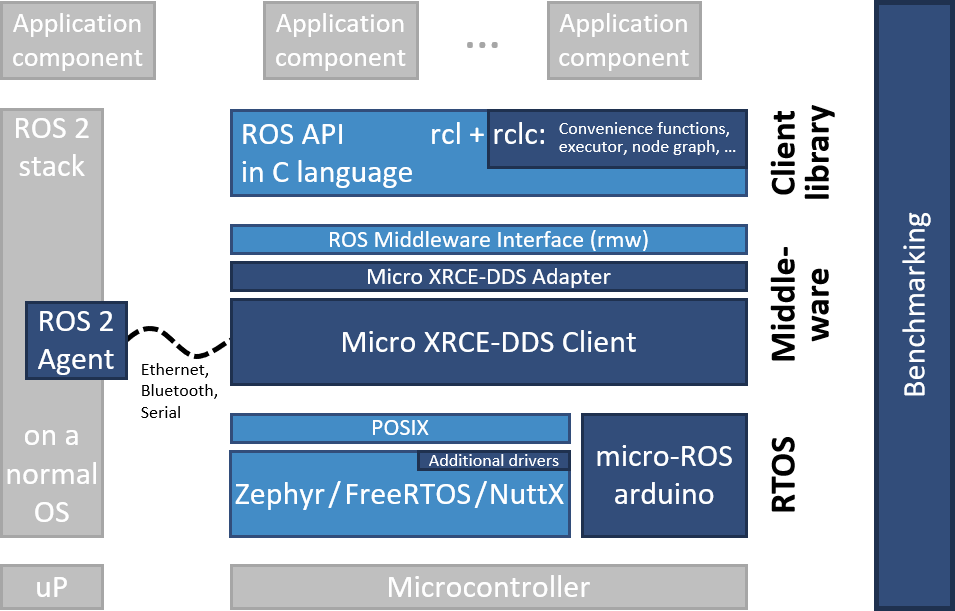
\includegraphics[width=0.8\textwidth]{imgs/Grundbegriffe/micro-ROS_architecture.png}
            \caption{Micro-ROS Architektur}
            \label{fig:micro-ros-architecture}%
        \end{figure}
    \end{description}
\end{flushleft}

\begin{flushleft}
    \textit{Technologischer Standpunkt Hardware:} \\
    Es existieren bereits viele Forschungen und Beispiele für diverse Roboter
    und deren verschiedensten Antriebskinematiken.
    Für unser Projekt werden wir allerdings eine eigene Roboter Platform designen und 3D-Drucken.
    Viele der bereits vorhandenen Roboter sind entweder zu Groß und teuer oder viel zu klein und deshalb ebenfalls nicht 
    gut für eine demonstration geeignet. Unter anderem wollen wir das unser Roboter den Vorteil bietet weitestgehend
    3D-gedruckt zu sein.
    Die ETH Zürich (TODO LINK?) hat bereits eine kleine Zusammenfassung über die wichtigsten Antriebsarten mobiler Roboter zur Verfügung gestellt.
    Für unser Projekt haben wir uns vorerst für einen simplen Diferentialantrieb entschieden. 
\end{flushleft}